\subsection*{Описание используемых данных}
\addcontentsline{toc}{subsection}{Описание используемых данных}

В нашем исследовании мы использовали открытый набор данных MTS Kion Implicit Contextualised Sequential Dataset for Movie Recommendation. Он включает 5 476 251 запись о взаимодействиях 962 179 пользователей с 15 706 фильмами. Для каждого сеанса просмотра в нём указаны метка времени, продолжительность и процент досмотра. Кроме того, датасет содержит демографические сведения о пользователях (пол, возраст, уровень дохода, наличие детей) и подробные метаданные о фильмах — жанры, ключевые слова, актерский состав, режиссеры и другие характеристики.

Датасет состоит из трех основных файлов:
\begin{itemize}
    \item \texttt{Interactions.csv} - фиксирует неявные взаимодействия пользователей с контентом, включая долю и время просмотра.
    \item \texttt{Users.csv} - включает демографические характеристики пользователей (пол, возрастная категория, доходы, наличие детей).
    \item \texttt{Items.csv} - содержит метаданные контента (название, оригинальное название, год производства, жанры, ключевые слова, описания, страны и студии производства, актерский состав, режиссеры).
\end{itemize}

Ключевые статистики датасета:
\begin{itemize}
    \item Количество пользователей: 962,179
    \item Количество объектов (фильмов): 15,706
    \item Количество взаимодействий: 5,476,251
    \item Среднее количество взаимодействий на одного пользователя: 5.69
    \item Разреженность данных: 99.9\%
\end{itemize}

\subsection*{Предобработка данных}
\addcontentsline{toc}{subsection}{Предобработка данных}
В ходе работы была выполнена предварительная обработка трех основных наборов данных (users, items, interactions) и данных для сабмита с использованием библиотеки polars. Ключевые этапы включали:
\begin{itemize}
    \item \textbf{Анализ и обработка пропущенных значений}: 
    Для каждого датафрейма были выявлены и обработаны пропуски. В категориальных признаках (например, возраст, пол, доход пользователей; оригинальное название, страны, студии у объектов) пропуски заменялись специальными метками (например, "age non specified", "Unknown") или наиболее подходящими значениями на основе анализа данных (например, 0 для watched pct или for kids).
    \item \textbf{Преобразование типов данных}:
    Многие колонки были преобразованы в более эффективные или семантически корректные типы. Категориальные строковые признаки (возраст, пол, доход, тип контента, жанры и др.) были переведены в тип Enum для оптимизации памяти и производительности. Числовые флаги (например, kids flg) преобразованы в булев тип. Даты (last watch dt) были переведены в формат Datetime.
    \item \textbf{Стандартизация текстовых данных}:
    Текстовые поля, такие как названия фильмов (title, title orig), стран, студий, режиссеров и актеров, были приведены к нижнему регистру и очищены от лишних пробелов. Для полей с множественными значениями (например, 'countries', 'studios') была применена стандартизация путем разделения, уникализации, сортировки и объединения значений.
    \item \textbf{Инженерия признаков}:
    На основе года выпуска фильмов (release year) был создан новый категориальный признак release year range, группирующий фильмы по десятилетиям.
    \item  \textbf{Проверка целостности}:
    После всех преобразований была выполнена проверка на отсутствие пропущенных значений в обработанных датафреймах.
    \item  \textbf{Сохранение результатов}:
    Очищенные и предобработанные датафреймы (users, items, interactions) были сохранены в эффективном формате Parquet для дальнейшего использования в исследовании.

    В целом, предобработка была направлена на улучшение качества данных, их консистентности и пригодности для последующего анализа и моделирования.
\end{itemize}

\subsection*{Создание текстовых эмбеддингов}
\addcontentsline{toc}{subsection}{Создание текстовых эмбеддингов}

Последующей задачей после предобработки данных является создание текстовых эмбеддингов каждого фильма. Для этого мы первым делом должны создать уникальное текстовое описание для каждого фильма. Для этого мы используем следующие поля:
\begin{itemize}
    \item \textbf{title}: Название фильма
    \item \textbf{genres}: Жанры фильма
    \item \textbf{kw}: Ключевые слова фильма
    \item \textbf{plot}: Описание фильма
    \item \textbf{countries}: Страны производства
    \item \textbf{studios}: Студии, производящие фильм
    \item \textbf{actors}: Актеры, сыгравшие в фильме
    \item \textbf{age rating}: Возрастной рейтинг фильма
\end{itemize}

Примером такого описания может служить следующий текст:
\begin{minted}[fontsize=\small,frame=single,label=Пример текстового описания фильма]{text}
title: поговори с ней
genres: драмы, зарубежные, детективы, мелодрамы
kw: трагедия, любовь, комедия, легендарный, педро
plot: мелодрама легендарного педро альмодовара
directors: педро альмодовар
actors: адольфо фернандес, ана фернандес, 
release_year: 2000-2010
age_rating: 16.0
\end{minted}

Первоначальный анализ существующих ключевых слов в датафрейме items df показал их неоптимальность для задачи создания эмбеддингов из-за дублирования информации из других полей (например, страна выпуска) и не всегда корректного разделения фраз.

Для решения этой проблемы было принято решение сгенерировать новые, более релевантные ключевые слова с помощью большой языковой модели (LLM). В качестве LLM была выбрана модель google/gemma-3-4b-it. Для генерации ключевых слов был разработан специальный промпт, состоящий из системного сообщения (SYSTEM MSG), инструктирующего модель выступать в роли эксперта-аналитика фильмов, и пользовательского промпта (build user prompt), который передавал модели название фильма (оригинальное и локализованное), жанры и описание. Инструкции для модели включали:

\begin{itemize}
    \item Сгенерировать до 8-10 ключевых слов или коротких фраз.
    \item Сфокусироваться на темах, сеттинге и атмосфере контента.
    \item Избегать общих слов (фильм, сериал, год, актеры).
    \item Выводить результат в виде списка, разделенного запятыми.
\end{itemize}

Генерация производилась батчами по 64 объекта для эффективности. Для каждого объекта формировался полный промпт, токенизировался, и модель model.generate создавала новые ключевые слова с параметрами max new tokens=50, do sample=True, temperature=0.3. Сгенерированные ключевые слова (generated\_keywords) были добавлены в исходный датафрейм items df в колонке kw.

На основе логики создания эмбеддингов, описанной раннее, а также сгенерированных ключевых слов было создано единое текстовое описание для каждого объекта, предназначенное для последующего получения векторных представлений (эмбеддингов).

Для преобразования текстовых описаний embedding\_text в векторные представления использовалась модель SentenceTransformer 'jina embeddings v3'. Это многоязычная многозадачная модель текстовых эмбеддингов, предназначенная для широкого спектра задач обработки естественного языка. Модель основана на архитектуре Jina-XLM-RoBERTa. Эмбеддинги генерировались батчами по 256 текстов, с последующей нормализацией и преобразованием в numpy массивы типа float32. Из полных эмбеддингов были отобраны первые 256 компонент для каждого объекта (emb\_256) для последующей кластеризации.

Качество полученных 256-мерных эмбеддингов оценивалось на основе их способности группировать семантически схожие объекты, используя жанровую информацию в качестве прокси-меры.
Была рассчитана матрица косинусного сходства (sim) между всеми парами эмбеддингов объектов. Для каждого объекта было найдено K=10 ближайших соседей.

Метрики оценки включали:
\begin{itemize}
    \item \textbf{Genre Hit-Rate@10}: Доля объектов, у которых хотя бы один из 10 ближайших соседей разделяет общий жанр. Полученное значение составило 0.987.
    \item \textbf{Mean Intra-Genre Similarity}: Среднее косинусное сходство между парами объектов, принадлежащих одному и тому же жанру. Это значение (0.400) сравнивалось со средним сходством между случайными парами объектов из разных кластеров (Mean inter sim = 0.282), что подтвердило хорошую семантическую группировку эмбеддингов. Дополнительно была проведена выборочная ручная проверка нескольких кластеров (на данном этапе еще не формализованных, а основанных на ближайших соседях) путем анализа их текстовых описаний.
\end{itemize}

\subsection*{Иерархическая кластеризация}
\addcontentsline{toc}{subsection}{Иерархическая кластеризация}

Для дальнейшего анализа и кластеризации объектов был использован алгоритм иерархической кластеризации. В качестве меры близости использовалось расстояние между эмбеддингами
\begin{itemize}
    \item \textbf{Построение k-NN графа}: Эмбеддинги объектов были L2-нормализованы. С использованием библиотеки faiss был создан индекс IndexFlatIP для эффективного поиска ближайших соседей по скалярному произведению (эквивалентно косинусному сходству для нормализованных векторов). Для каждого объекта было найдено K=50 ближайших соседей. На основе этой информации был сформирован датафрейм edges, представляющий собой k-NN граф с указанием источника (src), цели (dst) и косинусного сходства (cosine).

    \item \textbf{Учет "трафика" объектов}: Из датафрейма взаимодействий (interactions) для каждого item\_id был рассчитан 'трафик' как сумма общей длительности просмотров (total\_dur). Эти данные были сохранены в словаре traffic\_map.

    \item \textbf{Алгоритм balanced-split}: Был реализован рекурсивный алгоритм иерархической кластеризации. Целевое количество кластеров L2 было установлено в 320 (TARGET L2), максимальная глубина дерева – 9 (MAX DEPTH), максимальное и минимальное количество объектов в листовом кластере – 120 (MAX ITEMS) и 6 (MIN ITEMS) соответственно. Алгоритм итеративно разделял группы объектов на два подкластера с помощью KMeans (примененного к эмбеддингам), пока не достигались критерии остановки: максимальная глубина, целевой суммарный трафик листа или минимальное количество объектов в листе.

    \begin{algorithm}
    \caption{Алгоритм balanced-split кластеризации}
    \label{alg:balanced_split}
    \small
    \begin{algorithmic}[1]
    \Procedure{BalancedSplit}{$ids$, $traffic$, $vecs$, $L2$, $D$, $MAX$, $MIN$}
    \State $trf \gets \sum_{i \in ids} traffic.get(i)$; $max\_trf \gets trf / L2$
    \State $id2idx \gets \{id: idx \text{ for } (idx, id) \text{ in } enumerate(ids)\}$
    \State $clusters \gets \emptyset$; $stack \gets [(ids, 0)]$
    \While{$stack$ не пуст}
        \State $(nodes, depth) \gets stack.pop()$
        \State $leaf\_trf \gets \sum_{n \in nodes} traffic.get(n)$
        \If{$(depth = D)$ \textbf{or} $(leaf\_trf \leq max\_trf \text{ and } |nodes| \leq MAX)$ \textbf{or} $(|nodes| \leq MIN)$}
            \State добавить $nodes$ в $clusters$; \textbf{continue}
        \EndIf
        \State $X \gets vecs[[id2idx[n] \text{ for } n \in nodes]]$
        \State $labels \gets \Call{KMeans}{X, k=2}$
        \State $left, right \gets$ разделить $nodes$ по $labels$
        \If{$left$ пуст \textbf{or} $right$ пуст}
            \State добавить $nodes$ в $clusters$
        \Else
            \State $stack.append((left, depth + 1)); stack.append((right, depth + 1))$
        \EndIf
    \EndWhile
    \State \textbf{return} $clusters$
    \EndProcedure
    \end{algorithmic}
    \end{algorithm}
\end{itemize}

В результате было сформировано 249 кластеров L2 (листовых кластеров).
Пример одного из полученных кластеров:

\begin{quote}
\textbf{Кластер 124} | размер=99
\begin{itemize}
    \item \textit{пламя - я твоя тень} — жанры: драмы; ключевые слова: первобытный мир, огонь, борьба за выживание, примитивная пара, драка, выжив...
    \item \textit{таинственный сад} — жанры: семейное, фэнтези, приключения; ключевые слова: таинственный сад, магическое место, детство, приключе...
    \item \textit{ковчег} — жанры: приключения, детективы, драмы, зарубежные, фантастика; ключевые слова: фантастический сериал, ковчег, полярная...
    \item \textit{наваждение} — жанры: драмы, триллеры, детективы; ключевые слова: потеря, горе, спасение заложников, двойник, подозрение, италия...
\end{itemize}
\end{quote}

Что касается основных метрик кластеризации, то они получились следующими:
\begin{itemize}
    \item Коэффициент вариации "трафика" по кластерам составил 0.56, указывая на приемлемую сбалансированность.
    \item Среднее внутрикластерное косинусное сходство (0.453) оказалось заметно выше межкластерного (0.282), что свидетельствует о хорошем качестве разделения.
    \item Также был проведен ручной анализ содержимого нескольких случайных кластеров.
\end{itemize}

\subsection*{Извлечение ключевых слов кластеров}
\addcontentsline{toc}{subsection}{Извлечение ключевых слов кластеров}
Для каждого из 249 полученных L2 кластеров были извлечены характеризующие их ключевые слова.

\begin{itemize}
    \item Загружен датафрейм с результатами предыдущего этапа.
    \item В качестве текстовой основы для каждого объекта использовалась колонка core\_text (алиас для generated\_keywords, полученных от LLM).
    \item Тексты core\_text всех объектов внутри одного кластера были объединены в единый документ для этого кластера.
    \item Для каждого такого документа кластера с помощью TfidfVectorizer (с токенизацией nltk.word\_tokenize для русского языка, n-граммами (1, 2), min\_df=2, max\_features=50000) были рассчитаны TF-IDF веса слов и фраз.
    \item Для каждого кластера L2 были отобраны топ-5 ключевых слов/фраз с наибольшими TF-IDF значениями.
\end{itemize}

\subsection*{Подготовка данных для моделирования переходов между кластерами}
\addcontentsline{toc}{subsection}{Подготовка данных для моделирования переходов между кластерами}

На основе полученных кластеров и данных о взаимодействиях пользователей был сформирован датасет для задачи предсказания следующего кластера, который может заинтересовать пользователя.

\begin{itemize}
    \item Загружены данные о взаимодействиях пользователей и ключевых словах кластеров.
    \item Взаимодействия были отфильтрованы по проценту просмотра (watched pct >= 70).
    \item Для каждого пользователя была построена временная последовательность уникальных кластеров L2, с которыми он взаимодействовал.
    \item На основе этих последовательностей были созданы примеры для обучения: "промпт", содержащий ключевые слова двух предыдущих кластеров в последовательности, и "таргет" – ключевые слова следующего кластера в последовательности.
    \item Полученный датасет был сбалансирован путем ограничения количества примеров (до 10) для каждого уникального таргет-кластера, чтобы уменьшить влияние наиболее популярных кластеров. Изначальный размер 1,188,204 записей был сокращен до 2,449.
\end{itemize}

Пример полученного промпта для модели:

\begin{figure}[h]
\centering
\begin{tcolorbox}[
    colback=gray!5,
    colframe=gray!50,
    boxrule=1pt,
    arc=2pt,
    left=10pt,
    right=10pt,
    top=10pt,
    bottom=10pt,
    width=0.9\textwidth
]
\small\ttfamily
The films or series I watched most recently are in the following clusters:

\textbf{Cluster 1:} каледония, новая каледония, океан, биоразнообразие, гондурас

\textbf{Cluster 2:} индонезия, гондурас, природа, папуа, леса

Each cluster is described with salient phrases or entity names.
With less than 30 words, generate a new and different cluster I will watch next
with highly specific salient phrases or entity names, with a prefix that says "New cluster: "

\textbf{New cluster:} южная африка, африка, южная, дикая, дикая природа
\end{tcolorbox}
\caption{Пример промпта для модели предсказания следующего кластера.}
\label{fig:prompt_example}
\end{figure}

\section*{Моделирование переходов между кластерами}
\addcontentsline{toc}{section}{Моделирование переходов между кластерами}
Далее рассмотрим процесс дообучения большой языковой модели на сформированных промптах переходов между кластерами контента. Основная цель данного этапа заключается в адаптации предобученной модели к специфике задачи предсказания пользовательских предпочтений в области видеоконтента.

Для решения поставленной задачи был выбран подход fine-tuning существующей языковой модели, что позволяет использовать накопленные знания о языке и семантических связях, одновременно специализируя модель под конкретную предметную область. В качестве базовой архитектуры была выбрана модель "meta-llama/Llama-3.1-8B-Instruct", которая представляет собой инструкционно-настроенную версию модели Llama 3.1 с 8 миллиардами параметров.

Выбор данной модели обусловлен несколькими факторами:

\begin{itemize}
    \item Высокая эффективность в задачах следования инструкциям и генерации структурированного текста.
    \item Размер модели в 8 миллиардов параметров обеспечивает оптимальный баланс между качеством генерации и вычислительными требованиями.
    \item Открытая лицензия позволяет проводить дообучение и модификацию модели для исследовательских целей.
\end{itemize}

Процесс дообучения осуществляется на подготовленном датасете промптов переходов, где каждый пример содержит описание двух предыдущих кластеров в истории просмотров пользователя и целевой кластер, который пользователь выбрал следующим. Такая структура данных позволяет модели изучить паттерны пользовательского поведения и семантические связи между различными типами контента. Примеры сформированных промптов представлены на рисунке \ref{fig:prompt_example}.

\subsection*{Архитектура LoRA для эффективного дообучения}
\addcontentsline{toc}{subsection}{Архитектура LoRA для эффективного дообучения}

Для дообучения языковой модели Llama-3.1-8B-Instruct была применена архитектура LoRA (Low-Rank Adaptation), которая представляет собой эффективный метод параметрически-эффективного обучения больших языковых моделей.

LoRA основана на гипотезе о том, что изменения весов предобученной модели во время дообучения имеют низкий внутренний ранг. Вместо обновления всех параметров модели, LoRA добавляет обучаемые матрицы низкого ранга к существующим весам линейных слоев.

Для линейного слоя с весовой матрицей $W_0$, LoRA представляет обновление весов как:

\begin{equation}
W = W_0 + \Delta W = W_0 + BA
\end{equation}

где $B$ и $A$ — обучаемые матрицы низкого ранга $r$.

Основные преимущества LoRA:
\begin{itemize}
    \item Значительное сокращение количества обучаемых параметров
    \item Отсутствие дополнительной задержки во время инференса
    \item Возможность быстрого переключения между различными адаптерами
\end{itemize}

В нашем эксперименте использовались следующие параметры:
\begin{itemize}
    \item Ранг адаптации: $r = 16$
    \item Масштабирующий фактор: $\alpha = 32$
    \item Целевые модули: слои внимания и выходные проекции
\end{itemize}

Применение LoRA позволило сократить количество обучаемых параметров с 8,198,033,408 до 167,772,160 (2.05\% от общего количества), при этом сохранив высокое качество дообучения для задачи предсказания пользовательских предпочтений
Для обучения такого количества параметров была использована GPU Nvidia A100 40GB.

\subsection*{Параметры дообучения}
\addcontentsline{toc}{subsection}{Параметры дообучения}

Для дообучения модели были использованы следующие ключевые параметры:

\begin{itemize}
    \item \textbf{Размер батча}: 20 примеров на устройство с накоплением градиента через 2 шага (эффективный batch size = 40)
    \item \textbf{Количество эпох}: 10
    \item \textbf{Скорость обучения}: $2 \times 10^{-4}$ с разогревом в течение 10\% шагов
    \item \textbf{Оптимизатор}: AdamW
    \item \textbf{Точность вычислений}: bfloat16 для экономии памяти
    \item \textbf{Максимальная длина последовательности}: 512 токенов
    \item \textbf{Метрика для выбора лучшей модели}: article\_match\_rate
\end{itemize}

\subsection*{Метрики оценки модели}
\addcontentsline{toc}{subsection}{Метрики оценки модели}

Для оценки производительности дообученной языковой модели в задаче генерации рекомендаций следующего кластера интересов пользователя были использованы следующие метрики:

\textbf{1. recall\_exact\_completion (Точность полного совпадения)}

Данная метрика измеряет долю случаев, в которых текстовое описание кластера, сгенерированное моделью, полностью и дословно совпадает с эталонным описанием следующего кластера из тестового набора данных.

\begin{equation}
\text{recall\_exact\_completion} = \frac{N_{\text{полных совпадений}}}{N_{\text{всего примеров}}}
\end{equation}

где $N_{\text{полных совпадений}}$ — количество примеров, для которых предсказание модели идентично эталону, а $N_{\text{всего примеров}}$ — общее количество примеров в тестовом наборе. Метрика отражает способность модели к точному воспроизведению целевых последовательностей.

\textbf{2. avg\_jaccard\_to\_true (Средняя схожесть по ключевым словам с эталоном)}

Эта метрика оценивает среднюю степень семантического пересечения между набором ключевых слов, извлеченных из сгенерированного моделью описания кластера, и набором ключевых слов из эталонного описания кластера.

Для каждого примера извлекаются множества ключевых слов из предсказания модели ($K_{pred}$) и из эталона ($K_{true}$). Вычисляется индекс Жаккара:

\begin{equation}
J(K_{pred}, K_{true}) = \frac{|K_{pred} \cap K_{true}|}{|K_{pred} \cup K_{true}|}
\end{equation}

Итоговая метрика является средним значением индекса Жаккара по всем примерам тестового набора:

\begin{equation}
\text{avg\_jaccard\_to\_true} = \frac{1}{N_{\text{всего примеров}}} \sum_{i=1}^{N_{\text{всего примеров}}} J(K_{pred, i}, K_{true, i})
\end{equation}

Метрика характеризует, насколько предложенные моделью ключевые слова релевантны ожидаемым.

\textbf{3. article\_match\_rate (Соответствие критериям статьи)}

Ключевая метрика, оценивающая соответствие предсказания модели двум основным критериям: предложенный кластер должен быть (а) семантически отличным от двух предыдущих кластеров, показанных пользователю, и (б) семантически схожим с одним из существующих в системе валидных кластеров.

Для каждого примера:
\begin{itemize}
    \item Извлекается набор ключевых слов из предсказания модели ($K_{pred}$)
    \item Из промпта извлекаются наборы ключевых слов для двух предыдущих кластеров ($K_{prev1}$, $K_{prev2}$)
    \item Проверяется условие отличия: 
    \begin{align}
    J(K_{pred}, K_{prev1}) &< \text{порог}_{\text{отличия}} \text{ И} \\
    J(K_{pred}, K_{prev2}) &< \text{порог}_{\text{отличия}}
    \end{align}
    (например, $\text{порог}_{\text{отличия}} = 0.8$)
    \item Проверяется условие валидности: существует хотя бы один кластер $K_{valid}$ из общего списка валидных кластеров системы, для которого $J(K_{pred}, K_{valid}) \geq \text{порог}_{\text{валидности}}$ (например, $\text{порог}_{\text{валидности}} = 0.8$)
\end{itemize}

Если оба условия (отличие и валидность) выполнены, предсказание засчитывается как "match". Итоговая метрика:

\begin{equation}
\text{article\_match\_rate} = \frac{N_{\text{article matches}}}{N_{\text{всего примеров}}}
\end{equation}

Эта метрика отражает способность модели предлагать пользователю новые и одновременно релевантные интересы, соответствующие известным категориям.

\subsection*{Результаты дообучения}
\addcontentsline{toc}{subsection}{Результаты дообучения}

В процессе дообучения модели, как уже было отмечено, отслеживались ключевые метрики качества на валидационном наборе данных. Получившиеся результаты обучения представлены в таблице \ref{tab:training_results}.

\begin{table}[H]
\centering
\caption{Результаты дообучения модели по шагам}
\label{tab:training_results}
\small
\begin{tabular}{|c|c|c|c|c|}
\hline
\textbf{Шаг} & \textbf{Train Loss} & \textbf{Match Rate} & \textbf{Recall} & \textbf{Jaccard} \\
\hline
100 & 0.0779 & 0.9531 & 0.1694 & 0.2407 \\
\hline
200 & 0.0568 & 0.9918 & 0.3510 & 0.4058 \\
\hline
300 & 0.0496 & 0.9959 & 0.3857 & 0.4326 \\
\hline
400 & 0.0471 & 0.9939 & 0.3918 & 0.4394 \\
\hline
\end{tabular}
\end{table}

Анализ результатов показывает следующее:

\begin{itemize}
    \item \textbf{Снижение training loss}: Наблюдается устойчивое снижение потерь на обучающем наборе с 0.0779 до 0.0471, что свидетельствует об эффективном обучении модели.
    
    \item \textbf{Стабильность validation loss}: Потери на валидационном наборе остаются относительно стабильными (около 0.45), что указывает на отсутствие переобучения.
    
    \item \textbf{Высокие значения Article Match Rate}: Ключевая метрика достигает хороших результатов — от 95.3\% на 100-м шаге до 99.6\% на 300-м шаге, демонстрируя способность модели генерировать семантически корректные и отличающиеся от предыдущих кластеры.
    
    \item \textbf{Улучшение точности воспроизведения}: Метрика Recall Exact Completion показывает рост с 16.9\% до 39.2\%, отражая повышение способности модели к точному воспроизведению целевых описаний.
    
    \item \textbf{Рост семантической схожести}: Средний индекс Жаккара увеличивается с 0.24 до 0.44, что указывает на улучшение качества генерируемых ключевых слов.
\end{itemize}

\textbf{Пример работы модели}

Для демонстрации качества генерируемых рекомендаций приведем пример взаимодействия с дообученной моделью:

\begin{figure}[H]
\centering
\begin{tcolorbox}[
    colback=gray!5,
    colframe=gray!50,
    boxrule=1pt,
    arc=2pt,
    left=10pt,
    right=10pt,
    top=10pt,
    bottom=10pt,
    width=0.9\textwidth
]
\small\ttfamily
\textbf{Prompt:} The films or series I watched most recently are in the following clusters:

\textbf{Cluster 1:} война, отечественная война, отечественная, великая отечественная, летчики

\textbf{Cluster 2:} месть, драма, боевик, бои, спорт

Each cluster is described with salient phrases or entity names.
With less than 30 words, generate a new and different cluster I will watch next
with highly specific salient phrases or entity names, with a prefix that says "New cluster: "

\textbf{Предсказание:} New cluster: расследование, разруха, убийство, смоленск, советский детектив
\end{tcolorbox}
\caption{Пример работы дообученной модели.}
\label{fig:model_example}
\end{figure}

Данный пример демонстрирует способность модели генерировать семантически связанные, но отличающиеся от исходных кластеры, учитывая предпочтения пользователя к военной тематике и драматическим произведениям.

\subsection*{Создание lookup-таблицы для инференса}
\addcontentsline{toc}{subsection}{Создание lookup-таблицы для инференса}

После успешного дообучения модели следующим шагом стало создание эффективного механизма для практического применения модели в условиях реального времени. Для этого была разработана lookup-таблица, содержащая предвычисленные предсказания для всех возможных пар предыдущих кластеров.

\textbf{Процесс создания lookup-таблицы}

Идея заключается в том, чтобы для каждой возможной комбинации двух предыдущих кластеров предсказать следующий кластер с помощью дообученной LLM и сохранить эти соответствия. Процесс включает следующие этапы:

\begin{itemize}
    \item \textbf{Генерация всех возможных пар}: Из полученных 249 кластеров L2 формируются все возможные комбинации пар $(cluster_i, cluster_j)$, где $i, j \in \{1, 2, ..., 249\}$.
    
    \item \textbf{Создание промптов}: Для каждой пары кластеров автоматически генерируется промпт в том же формате, который использовался при обучении модели.
    
    \item \textbf{Генерация предсказаний}: Дообученная модель обрабатывает каждый промпт и генерирует предсказание следующего кластера.
    
    \item \textbf{Сохранение соответствий}: Результаты сохраняются в виде таблицы соответствий вида $(cluster_{prev1}, cluster_{prev2}) \rightarrow cluster_{next}$.
\end{itemize}

\textbf{Архитектура предлагаемого пайплайна}

На основе созданной lookup-таблицы может быть разработан эффективный пайплайн рекомендательной системы:

\begin{figure}[H]
\centering
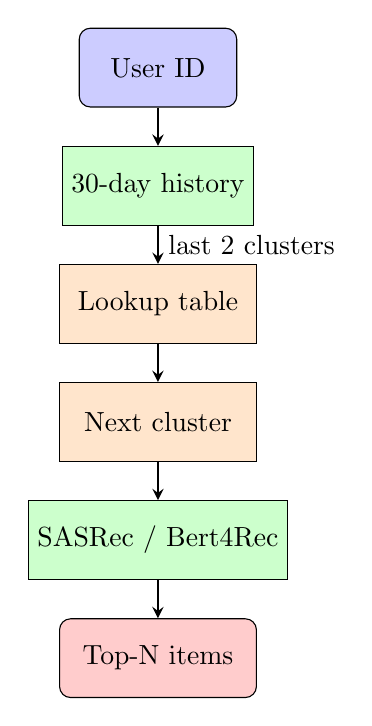
\begin{tikzpicture}[node distance=1.5cm]
    % Определение стилей
    \tikzset{
        start/.style={rectangle, rounded corners, minimum width=2cm, minimum height=1cm, text centered, draw=black, fill=blue!20},
        process/.style={rectangle, minimum width=2.5cm, minimum height=1cm, text centered, draw=black, fill=orange!20},
        decision/.style={rectangle, minimum width=2cm, minimum height=1cm, text centered, draw=black, fill=green!20},
        endpoint/.style={rectangle, rounded corners, minimum width=2.5cm, minimum height=1cm, text centered, draw=black, fill=red!20},
        arrow/.style={thick,->,>=stealth}
    }

    % Узлы
    \node (user) [start] {User ID};
    \node (history) [decision, below of=user] {30-day history};
    \node (lookup) [process, below of=history] {Lookup table};
    \node (cluster) [process, below of=lookup] {Next cluster};
    \node (mask) [decision, below of=cluster] {SASRec / Bert4Rec};
    \node (items) [endpoint, below of=mask] {Top-N items};

    % Стрелки
    \draw [arrow] (user) -- (history);
    \draw [arrow] (history) -- node[anchor=west] {last 2 clusters} (lookup);
    \draw [arrow] (lookup) -- (cluster);
    \draw [arrow] (cluster) -- (mask);
    \draw [arrow] (mask) -- (items);
\end{tikzpicture}
\caption{Схема предлагаемого пайплайна рекомендательной системы}
\label{fig:pipeline}
\end{figure}

Предлагаемый пайплайн должен работать следующим образом:

\begin{enumerate}
    \item \textbf{Извлечение истории пользователя}: По User ID получается 30-дневная история взаимодействий пользователя.
    
    \item \textbf{Определение последних кластеров}: Из истории выделяются уникальные последние 2 кластера, с которыми взаимодействовал пользователь.
    
    \item \textbf{Поиск в lookup-таблице}: По паре предыдущих кластеров в предвычисленной таблице находится рекомендуемый следующий кластер.
    
    \item \textbf{Применение SASRec}: Используется предобученная модель SASRec с маскированием логитов для генерации рекомендаций только из объектов целевого кластера.
    
    \item \textbf{Формирование рекомендаций}: Возвращается список Top-N наиболее релевантных объектов из предсказанного кластера.
\end{enumerate}

\textbf{Преимущества данного подхода}

Использование lookup-таблицы обеспечивает:

\begin{itemize}
    \item \textbf{Высокую скорость инференса}: Устраняется необходимость в реальном времени запускать тяжелую LLM для генерации предсказаний.
    
    \item \textbf{Предсказуемую латентность}: Время отклика системы становится константным и не зависит от сложности модели.
    
    \item \textbf{Масштабируемость}: Система может обслуживать большое количество пользователей одновременно без дополнительных вычислительных затрат на LLM.
    
    \item \textbf{Простоту развертывания}: Не требуется специализированная инфраструктура для запуска больших языковых моделей в продакшене.
\end{itemize}

Полученные результаты подтверждают эффективность применения LoRA-архитектуры для дообучения большой языковой модели в задаче генерации персонализированных рекомендаций контента, а также решению проблемы замкнутости рекомендательной системы.

\textbf{Направления дальнейших исследований}

Следующим этапом исследования было бы проведение онлайн-эксперимента для сравнения производительности дообученной языковой модели с классическими подходами к рекомендациям. В качестве базовых методов для сравнения целесообразно рассмотреть:

\begin{itemize}
    \item \textbf{Hierarchical Contextual Bandit} — метод, использующий иерархическую структуру для моделирования контекстных предпочтений пользователей
    \item \textbf{Collaborative Filtering} — классические алгоритмы коллаборативной фильтрации
    \item \textbf{Content-based методы} — рекомендации на основе содержательных характеристик объектов
    \item \textbf{Гибридные подходы} — комбинирующие различные методы рекомендаций
\end{itemize}

Онлайн-тестирование позволило бы оценить реальное влияние предлагаемого подхода на пользовательский опыт, измерить метрики вовлеченности (время просмотра, количество кликов, конверсия) и проверить способность модели решать проблему замкнутости рекомендательных систем в реальных условиях эксплуатации.
